\documentclass[hidelinks]{article}
\usepackage[letterpaper,margin=1.0in]{geometry}
\usepackage[utf8]{inputenc}
\pagenumbering{arabic}
\usepackage{authblk}
\usepackage{graphicx}
\usepackage[singlelinecheck=false]{caption} % singlelinecheck makes single line caption left aligned instead of centered
\usepackage{subcaption}
\usepackage{amsmath}
\usepackage[round]{natbib}
\usepackage{fancyhdr}
\usepackage{longtable}
\usepackage{booktabs}
% hyperlinks
\usepackage{hyperref}

\usepackage{xspace}
\usepackage{mathrsfs}
\usepackage{graphicx}

\pagestyle{fancy}
\fancyhead[R]{\textbf{Expanding \stdpopsim}}

% for highlighting text
\usepackage{xcolor}
\usepackage{soul}

% bibliography
\usepackage[round]{natbib}   % omit 'round' option if you prefer square brackets
\bibliographystyle{plainnat}



\newcommand{\Stdpopsim}{\texttt{Stdpopsim}\xspace}
\newcommand{\stdpopsim}{\texttt{stdpopsim}\xspace}

%commands to format figure and table references in the supplement
\newcommand{\beginsupplement}{%
        \fancyhead[L]{Supplemental Material}
        \setcounter{table}{0}
        \renewcommand{\thetable}{S\arabic{table}}%
        \setcounter{figure}{0}
        \renewcommand{\thefigure}{S\arabic{figure}}%
     }
\newcommand{\stopsupplement}{%
        \setcounter{table}{0}
        \renewcommand{\thetable}{\arabic{table}}%
        \setcounter{figure}{0}
        \renewcommand{\thefigure}{\arabic{figure}}%
     }

\makeatletter
\newcommand{\labelname}[1]{\def\@currentlabelname{#1}}
\makeatother

% Avoid pandoc bug when there are lists in the body.
\providecommand{\tightlist}{%
\setlength{\itemsep}{0pt}\setlength{\parskip}{0pt}}

\title{Expanding the \stdpopsim species catalog, and lessons learned for realistic genome simulations}

\author[1,*]{M. Elise Lauterbur}
\author[2,*]{Maria Izabel A. Cavassim}
\author[3,*]{Ariella L. Gladstein}
\author[4,*]{Graham Gower}
\author[5,*]{Georgia Tsambos}
\author[6,7]{Jeff Adrion} % moved from above at request
\author[8]{Arjun Biddanda}
\author[6]{Saurabh Belsare}
\author[6]{Victoria Caudill}
\author[9]{Jean Cury}
\author[10]{Ignacio Echevarria}
\author[11,12]{Ahmed Hasan}
\author[13,14]{Xin Huang}
\author[15]{Leonardo Nicola Martin Iasi} % lastname Iasi
\author[16]{Jana Obšteter}
\author[17]{Vitor Antonio Corrêa Pavinato} % lastname Pavinato
\author[18,19]{David Peede}
\author[20]{Ekaterina Noskova}
\author[21,22]{Alice Pearson}
\author[23]{Manolo Perez}
\author[6]{Murillo F. Rodrigues}
\author[6]{Chris C. R. Smith}
\author[24]{Jeff Spence}
\author[6]{Anastasia Teterina}
\author[6]{Silas Tittes}
\author[25]{Per Unneberg}
\author[26]{Juan Manuel Vasquez}
\author[27]{Ryan Waples}
\author[28]{Anthony Wilder Wohns}
\author[29]{Yan Wong}
\author[30]{Reed Cartwright}
\author[31]{Aaron P. Ragsdale}
\author[32]{Franz Baumdicker}
\author[33]{Gregor Gorjanc}
\author[34]{Ryan N. Gutenkunst}
\author[29]{Jerome Kelleher}
\author[6]{Andrew D. Kern}
\author[6,35]{Peter L. Ralph}
\author[36]{Daniel R. Schrider}
\author[37]{Ilan Gronau}


\affil[*]{\small{These authors contributed equally to the paper.}}
\affil[1]{\small{Department of Ecology and Evolutionary Biology, University of Arizona, Tucson AZ 85719}}
\affil[2]{\small{Department of Ecology and Evolutionary Biology University of California, Los Angeles}}
\affil[3]{\small{Embark Veterinary, Inc., Boston, MA 02111, USA}}
\affil[4]{\small{Section for Molecular Ecology and Evolution, Globe Institute, University of Copenhagen, Denmark}}
\affil[5]{\small{School of Mathematics and Statistics, University of Melbourne, Australia}}
\affil[6]{\small{Institute of Ecology and Evolution, University of Oregon, Eugene OR 97402}}
\affil[7]{\small{AncestryDNA, San Francisco, CA, 94107, USA}}
\affil[8]{\small{54Gene, Inc., Washington, DC 20005, USA}}
\affil[9]{\small{Université Paris-Saclay, CNRS, INRIA, Laboratoire Interdisciplinaire des Sciences du Numérique, UMR 9015 Orsay, France}}
\affil[10]{\small{School of Life Sciences, University of Glasgow}}
\affil[11]{\small{Department of Computational Biology, Cornell University}}
\affil[12]{\small{Department of Cell and Systems Biology, University of Toronto, Toronto ON}}
\affil[13]{\small{Department of Biology, University of Toronto Mississauga, Mississauga ON}}
\affil[14]{\small{Department of Evolutionary Anthropology, University of Vienna, Djerassiplatz 1, 1030 Vienna, Austria}}
\affil[15]{\small{Human Evolution and Archaeological Sciences (HEAS), University of Vienna, Austria}}
\affil[16]{\small{Department of Evloutionary Genetics, Max Planck Institute for Evolutionary Anthropology, Leipzig, Germany}}
\affil[17]{\small{Agricultural Institute of Slovenia, Department of Animal Science, Hacquetova ulica 17, Ljubljana, Slovenia}}
\affil[18]{\small{Entomology Dept., CFAES, The Ohio State University, Wooster, Ohio}}
\affil[19]{\small{Department of Ecology and Evolutionary Biology, Brown University, Providence, RI, USA}}
\affil[20]{\small{Center for Computational Molecular Biology, Brown University, Providence, RI, USA}}
\affil[21]{\small{Computer Technologies Laboratory, ITMO University, St Petersburg, Russia}}
\affil[22]{\small{Department of Genetics, University of Cambridge, UK}}
\affil[23]{\small{Department of Zoology, University of Cambridge, UK}}
\affil[24]{\small{Department of Genetics and Evolution, Federal University of Sao Carlos, Sao Carlos 13565905, Brazil}}
\affil[25]{\small{Department of Genetics, Stanford University School of Medicine, Stanford, CA, 94305}}
\affil[26]{\small{Department of Cell and Molecular Biology, National Bioinformatics Infrastructure Sweden, Science for Life Laboratory, Uppsala University,  Husargatan 3, SE-752 37 Uppsala, Sweden}}
\affil[27]{\small{Department of Integrative Biology, University of California, Berkeley, Berkeley, CA, USA}}
\affil[28]{\small{Department of Biostatistics, University of Washington}}
\affil[29]{\small{Broad Institute of MIT and Harvard, Cambridge, MA 02142, USA}}
\affil[30]{\small{Big Data Institute, Li Ka Shing Centre for Health Information and Discovery, University of Oxford, OX3 7LF, UK}}
\affil[31]{\small{School of Life Sciences and The Biodesign Institute, Arizona State University, Tempe, AZ USA}}
\affil[32]{\small{Integrative Biology, University of Wisconsin-Madison, Madison, Wisconsin}}
\affil[33]{\small{Cluster of Excellence - Controlling Microbes to Fight Infections, Eberhard Karls Universität Tübingen, Tübingen, Baden-Württemberg, Germany}}
\affil[34]{\small{The Roslin Institute and Royal (Dick) School of Veterinary Studies, University of Edinburgh, Edinburgh EH25 9RG, UK}}
\affil[35]{\small{Department of Molecular and Cellular Biology, University of Arizona, Tucson, Arizona 85721}}
\affil[36]{\small{Department of Mathematics, University of Oregon, Eugene OR 97402}}
\affil[37]{\small{Department of Genetics, University of North Carolina at Chapel Hill, Chapel Hill, North Carolina 27599}}
\affil[38]{\small{Efi Arazi School of Computer Science, Reichman University, Herzliya, Israel}}

\date{\small{\today{}}}

\begin{document}

\maketitle


\section*{Abstract}

Simulation is a key tool in population genetics for both methods development and empirical research,
but producing simulations that recapitulate even the main features of genomic datasets remains a major obstacle.
Today, more realistic simulations are possible thanks to large increases in
the quantity of available data
and the sophistication of inference and simulation software,
but implementing these simulations can require substantial time and specialized knowledge.
These challenges are especially pronounced for simulating less well-studied species,
since it is not always clear what level of realism is sufficient
to confidently answer a given question, or what information is required
to produce simulations of that desired realism.
\Stdpopsim is a community-developed tool that seeks to lower this barrier
by making it easy to simulate complex population genetic models using
up-to-date information.
The initial version of the \stdpopsim catalog contained information for 
6 species, most of which are well-characterized model organisms.
Here, we report on community-driven efforts to expand the catalog 
more broadly across the tree of life, which now contains 21 species,
with 25 demographic models and 37 genetic maps.
The process of expanding the \stdpopsim catalog 
to include more species through community engagement yielded many insights, 
and we report on lessons learned for best practices in population genomic simulation.
We discuss the elements of a population genomic
simulation model, including the required input data, common pitfalls and major considerations,
and describe how new species models can be integrated into \stdpopsim.
We also introduce several major advances to the realism of \stdpopsim's simulation ability,
including gene conversion and provision of species-specific genomic annotations.
Together, these advances to \stdpopsim will strengthen efforts to use and develop
simulation-based population genomic inference methods, with particular advances
for non-model organisms, making them available, transparent, and accessible to everyone.




\section*{Introduction}
    \label{introduction}

%Simulation is one of the key tools in population genetics, but can
%present unexpected challenges and has many hidden pitfalls for the
%unwary population geneticist.

Dramatic reductions in sequencing costs are enabling the generation of
unprecedented amounts of genomic data for a huge variety of species
\citep{Ellegren2014}. Ongoing efforts to systematically sequence life on
Earth by initiatives such as the Earth Biogenome \citep{Lewin2022} and its
affiliated project networks (for example, Vertebrate Genomes
\citep{Rhie2021}, 10,000 Plants \citep{Cheng2018} and others \citep{darwin2022sequence}) are
providing the backbone for enormous increases in the amount of population-level genomic data
available for model and non-model species.
These data are being used to answer questions across scales
from deep evolutionary time to ongoing ecological dynamics.
Methods that use these data, for example to infer demographic history and natural selection,
are also flourishing \citep{Beichman2018}.
While past methods development focused on humans and a few key model systems such as \emph{Drosophila},
more recent efforts are generalizing these methods to include 
important population dynamics not initially accounted for,
such as inbreeding or selfing \citep{Blischak2020}, skewed offspring
distributions \citep{Montano2016}, and intense artificial selection \citep{MacLeod2013, MacLeod2014}.

Simulations can be useful at all stages of this work --
for planning studies, analyzing data, testing inference methods,
and validating findings from empirical and theoretical research.
For instance, simulations provide training data
for inference methods based on machine learning \citep{Schrider2018} and
Approximate Bayesian Computation \citep{Csillery2010}. They can also serve as
baselines for further analyses: for example, simulations incorporating
demographic history serve as null models when detecting selection \citep{Hsieh2016a}
or seed downstream breeding program simulations \citep{Gaynor2020}.
More recently, population genomic simulations have begun
to be used to help guide conservation decisions for threatened species
\citep{Teixeira2021,kyriazis2022using}.

Increasing amounts of data and sophistication of inference methods
have enabled researchers to ask ever more
specific and precise questions. Consequently, simulations must incorporate
more and more detailed elements of a species' biology.
Important elements include genomic features such as mutation and recombination
rates that strongly affect genetic variation and haplotype structure
\citep{Nachman2002}. These have particularly strong ramifications 
when linked selection is important in the patterns of genomic diversity being studied \citep{Cutter2013}.
Furthermore, the demographic history of a species,
encompassing population sizes and distributions, divergences, and gene flow, can
dramatically affect patterns of genomic variation \citep{Teshima2006}. Thus
species-specific estimates of these and other ecological and evolutionary parameters 
(e.g., those governing the process of natural selection) 
are fundamentally important when developing simulations.
This presents challenges, especially to new researchers,
as it takes a great deal of specialized knowledge not only to code the simulations themselves
but also to find and choose appropriate estimates of the parameters underlying the simulation model.

\Stdpopsim is a community resource recently developed to provide easy
access to detailed population genomic simulations \citep{Adrion2020}. It
lowers the technical barriers to performing these simulations
and reduces the possibility of erroneous implementation of simulations
for species with published demographic models. 
The initial release of \stdpopsim was
restricted to only six well-characterized model species, such as
\emph{Drosophila melanogaster} and \emph{Homo sapiens},
but feedback from \stdpopsim workshops identified a widespread desire
to simulate a wider range of non-model species,
and ideally to incorporate these into the \stdpopsim catalog for future use.
That feedback, and subsequent efforts to expand the catalog, 
also uncovered the need for a better understanding of when it is practical to create a realistic
simulation of a species of interest, and indeed what ``realistic'' means in this context.
In addition to \stdpopsim's framework for standardizing simulations of some species,
our experience has led us to develop guidance that may be of use to
the broader population genetics community.

This paper is intended to announce and describe the additions to the \stdpopsim catalog,
and as a resource for methods developers and empirical researchers
who wish to develop simulations of their own species of interest
or add to the \stdpopsim catalog.
In the \nameref{sec:sim-guidelines} section,
we discuss the elements of a
population genomic simulation model that characterizes a
species, including when a whole-genome simulation is more useful than
simulations based on either individual loci or generic (non-species specific) loci.
We discuss the required input data (genome assembly,
mutation and recombination rates, and demographic model),
common pitfalls in choosing appropriate parameters, and
considerations for species that are missing estimates of some
necessary inputs. This paper is not intended as a tutorial for
implementing simulations in any particular simulator, rather to provide
guidance for what information is sufficient for a realistic genome simulation
using any simulator. We pay particular attention to the ways
in which \stdpopsim eases this burden, and describe how new users might
add their own species information to \stdpopsim.
The latter is discussed in the \nameref{sec:examples} section, where we lay out in
detail the simple process of incorporating the information discussed
in the \nameref{sec:sim-guidelines} section into \stdpopsim.



\section*{The utility of \stdpopsim for genome-wide simulations}
    \label{sec:std-sim}
% Elise: This section feels disjoint without the sub-headings that are 
% currently commented out ("Parameterizing population genomic simulations
% is cumbersome," "Stdpopsim streamlines the parameterization of population genomic simulations,"
% "Species-specific genomic architecture is challenging to model.")
% The last section (genomic architecture) especially comes out of nowhere.
% I've made some efforts to mitigate that below, but it could use more attention.

% \paragraph*{Parameterizing population genomic simulations is cumbersome}
We begin with an overview of the goals and rationale behind \stdpopsim
and complete chromosome simulation;
see \citet{Adrion2020} for more on the topic.
The main objective of population genomic simulations is to recreate 
patterns of sequence variation along the genome under known conditions
that model a given species (or population) of interest.
\Stdpopsim is built on top of the
\texttt{msprime} \citep{Kelleher2016,Nelson2020,Baumdicker2022}
and \texttt{SLiM} \citep{Haller2019} simulation engines,
that are capable of producing fairly realistic patterns of sequence variation
if provided with accurate descriptions of the genome architecture
and evolutionary history of the simulated species.
The required parameters include the number of chromosomes and their lengths,
mutation and recombination rates, the demographic history of the simulated population,
and, potentially, the landscape of natural selection along the genome.
A key challenge when setting up a population genomic simulation is to
obtain estimates of all of these quantities from the literature
and then correctly implement them in an appropriate simulation engine.
Detailed estimates of all of these quantities are increasingly available
due to the growing availability of population genomic data
coupled with methodological advances. Incorporating this data
into a population genomic simulation often involves 
integrating this data between different literature sources, which can
require specialized knowledge of population genetics theory.
As a result, while the simulations themselves may require considerable computational resources,
the most time-consuming and error-prone part of population genomic simulation is
often the task of correctly parameterizing simulation software.

% \paragraph*{\Stdpopsim streamlines the parameterization of population genomic simulations}
The main objective of \stdpopsim is to streamline this process,
making it less time consuming, less error prone, and more reproducible.
Contributors use a template to build the model for their species of interest,
including the required parameter values. This model then goes through a
vital peer-review process, including validating the choices of parameter values.
% Elise: Commented out the below sentences because this seems like too much detail here. Replaced with above sentence.
% To ensure reliability,
% after a contributor adds a new simulation model to the catalog, it is flagged for review.
% Then, another contributor independently creates a simulation model
% based on the same literature sources and the documentation provided by the initial contributor.
% The two separate models are then compared to each other by automated scripts.
% Any discrepancies are resolved by the two contributors,
Any discrepancies are resolved between the contributor and reviewer,
if necessary with input of additional members of the community.
This quality control process quite often finds subtle bugs \citep[e.g., as in][]{Ragsdale2020}
or highlights parts of the model that are ambiguously defined by the literature sources.
This considerably increases the reliability of the resulting simulations in any downstream analysis.


% \paragraph*{\textbf{Species-specific genomic architecture is challenging to model}}
The goal of complete chromosome simulation is important for a number of reasons.
The organization of genes on chromosomes is a key feature of a species' genome,
and one that has largely been ignored in population genomic simulation (see \cite{schrider2020background} for a notable exception).
% DRS: I added a citation for one exception I could think of, but it is not especially notable. Any more we could add?
This is largely because simulation of chromosome-scale sequences, on the order of $ > 10^7$ bp,
has until recently been largely out of reach computationally, 
so population geneticists have resorted to separate simulations of many short segments
of the genome \citep[e.g.,][]{harris2016genetic}.

However, physical linkage of chromosomes induces correlations along a chromosome that
generally reduce variance relative to independent simulations of equivalent genetic material.
This has a particularly striking effect in long stretches of low recombination rates,
as observed for instance on the long arm of human chromosome 22 \citep{Dawson2002}.
When conducting simulations with natural selection, linkage has
an even stronger effect. Selection acting on a small number of sites can
indirectly influence levels and patterns of genetic variation at linked neutral sites,
which has been shown to have a widespread
effect on patterns of genome variation in myriad species
\citep[e.g.,][]{McVicker2009,Charlesworth2012}. 
In addition, the lengths of chromosome-scale shared haplotypes within and
between populations provides valuable information.
Methods that use such information, such as MSMC \citep{Schiffels2020},
or IBDNe \citep{browning2015accurate} %, or the method of \citet{ringbauer2018estimating},
perform best on long genomic segments, with realistic recombination rates.
Chromosome-scale simulations are clearly required to test (or, train) such methods,
or to conduct power analyses for design of empirical studies that use them.


% ILAN: commented out this part on genetic load. We can mention this briefly,
%   if we think it's important
%
%Third, linkage has the potential to affect demographic realism. The
%genetic load in a simulation of a small segment of chromosome with
%deleterious mutations will necessarily be less than that in whole
%chromosome. This situation makes it easy to simulate unrealistically
%high levels of load without realizing it, if only small unlinked segments are used.
%(TODO: What is the direct effect on demographic realism of the effect of
%load?) (DRS: I think that the three examples given in this section
%aren't the most compelling. The point of the chr22 example isn't super clear,
%the chromosome ends thing seems like a minor issue especially given that
%rec rates there are generally pretty low, and the load case seems to be
%more an issue of ``small scale sims let you simulate unrealistic secnarios''
%rather than ``small scale sims prevent you from simulating realistic scenarios''

% Andy: I'm commenting this out here to stay on message
% That said, for some purposes it might be completely fine to simulate short sequence
% segments or even independent (unlinked) sites. However, this should be done after
% careful consideration  of the benefits of whole-chromosome simulations.


\subsection*{Additions to \stdpopsim}
    \label{sec:expanded-catalog}

Since its initial publication in \cite{Adrion2020},
we have increased the number of species in the catalog nearly fourfold,
added multiple demographic models and genetic maps, and
improved the simulation framework of \stdpopsim in several ways.

When first published, the \stdpopsim catalog included six species:
\emph{Homo sapiens}, \emph{Pongo abelii}, \emph{Canis familiaris}, \emph{Drosophila melanogaster},
\emph{Arabidopsis thaliana}, and \emph{Escherichia coli} (Figure \ref{fig:tree}).
One way the catalog has expanded is through introduction of additional demographic models
for \emph{Homo sapiens}, \emph{Pongo abelii}, \emph{Drosophila melanogaster},
and \emph{Arabidopsis thaliana}, enabling a wider variety of simulations for these
mostly model species.

However,
these species represent a small slice of the tree of life.
This is a concern
not only because of the large community of researchers studying other organisms that might benefit from these efforts,
but also because methods developed for application to humans (for instance)
may not perform well when applied to other species with very different biology.
It should thus be made easy to test methods across a wide variety of organisms.
To begin to address this, we made a concerted effort
to recruit members of the population and evolutionary genetics community
to add new species to the \stdpopsim catalog, culminating in a
``Growing the Zoo'' hackathon organized alongside the 2021 ProbGen conference.
To introduce people to using \stdpopsim and to prepare people for the hackathon,
we organized a series of seven workshops in the preceeding months.
These allowed us to reach a broad community of more than 150 researchers,
many of whom expressed interest in adding non-model species to \stdpopsim.
The hackathon was then structured based on feedback from these participants.
One month before the hackathon, we organized a final workshop to prepare interested
participants for the hackathon, by introducing them to  the process of developing
a new species model and adding it to the \stdpopsim code base.

Roughly 20 scientists participated in the hackathon,
which resulted in the addition of 15 species to the \stdpopsim catalog
% % PLR: no need to split hairs here.
% This initial concentrated effort later resulted in the addition or refinement of
% of 3 more species during the year following the hackathon
(Figure \ref{fig:tree}).

\begin{figure}
    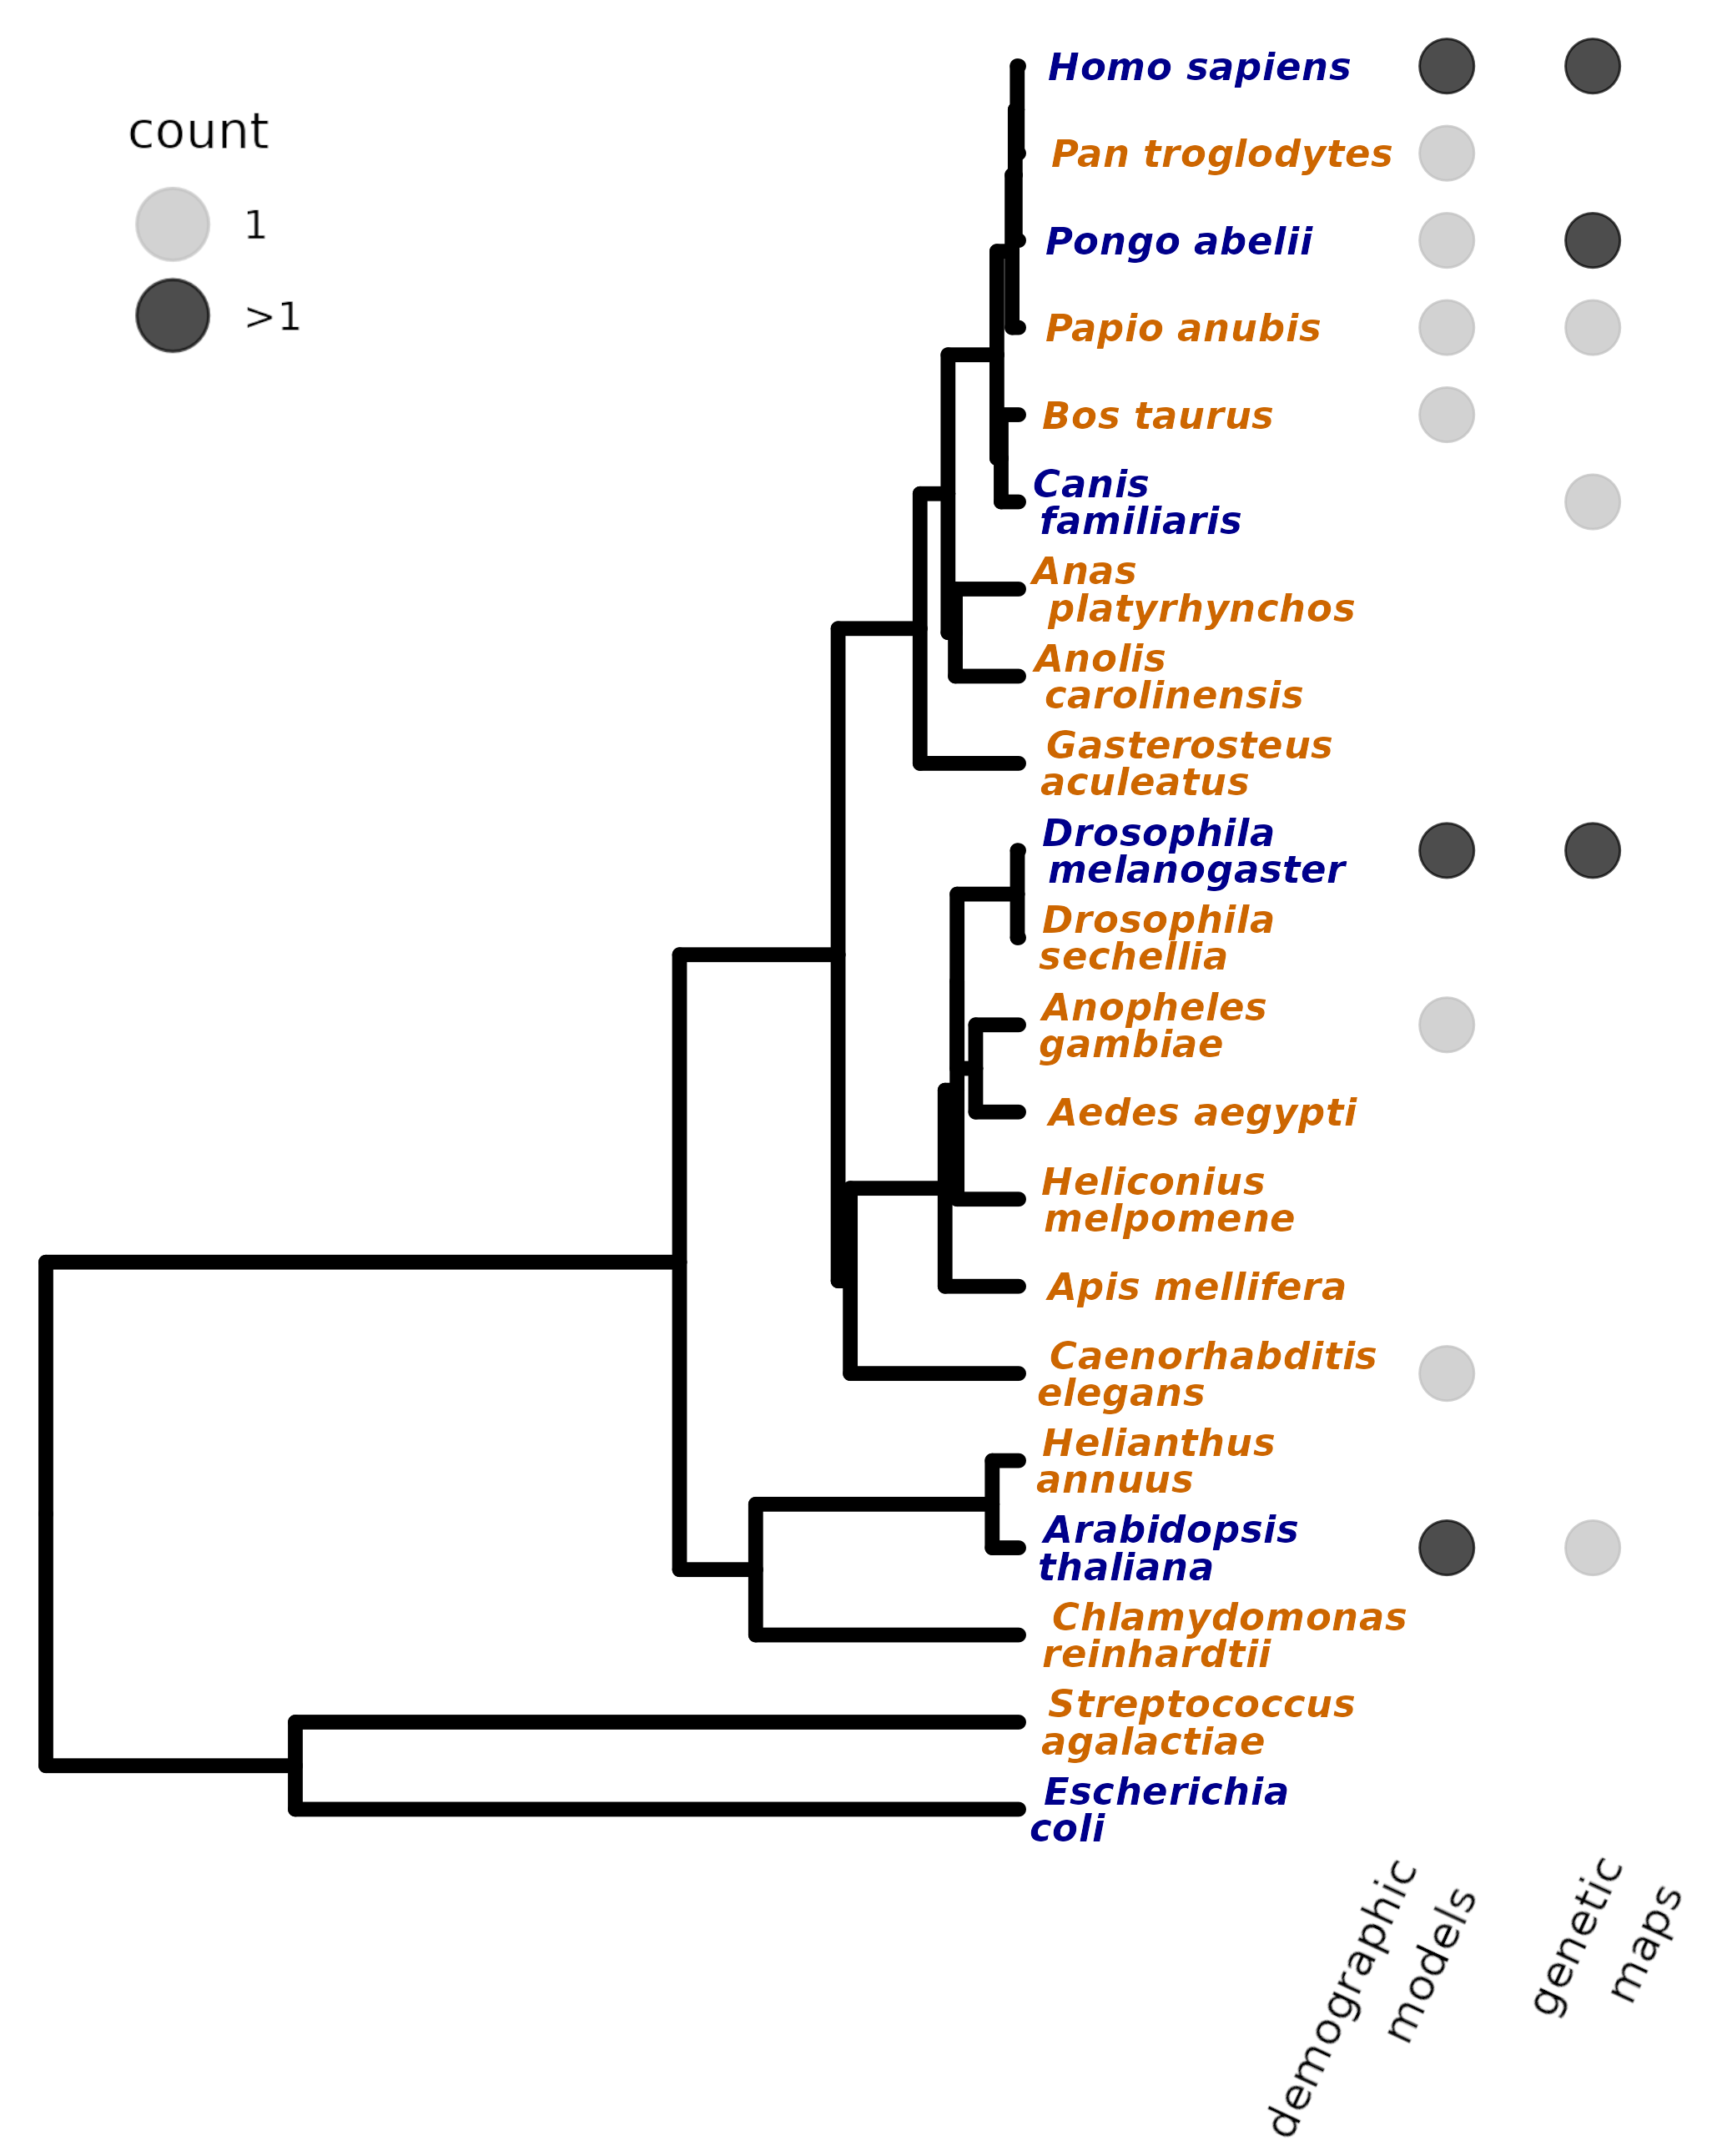
\includegraphics[width=\linewidth]{figs/species_fig}
	\caption{Phylogenetic tree of species available in the \stdpopsim catalog.
		In blue are species we published in the original release \citep{Adrion2020}, in orange are those 
		species that have since been added. Columns show which species have one (light grey) or more
		(dark grey) demographic models and genetic maps.
	\label{fig:tree} }
\end{figure}

The catalog now includes
a teleost fish (\textit{Gasterosteus aculeatus}),
a bird (\textit{Anas platyrhynchos}),
a reptile (\textit{Anolis carolinensis}),
a livestock species (\textit{Bos taurus}),
six insects including two vectors of human disease (\textit{Aedes aegypti} and \textit{Anopheles gambiae}),
a nematode (\textit{Caenorhabditis elegans}),
two flowering plants including a crop (\textit{Helianthus annuus}),
an algae (\textit{Chlamydomonas reinhardtii}),
and two bacteria,
in addition to four primates 
and a common mammalian associate of primates (\textit{Canis familiaris}). % Elise: An aside, I find this way of describing dogs to be hilariously academic
Not all of these have genetic maps or demographic models,
but this lays the framework for future contributions.

A key feature added to \stdpopsim that expands the diversity of species that can
be realistically modeled is the inclusion of recombination by gene conversion,
which is essential for organisms such as \textit{E.\ coli}
that lack crossing over.
\colorbox{yellow}{[ TODO: summarize model of GC (see PR\#57) ]}
% Elise: Not sure the blow fits in the GC paragraph?
In addition, the update to msprime version 1.0~\citep{Baumdicker2022}
provides a number of additional benefits such as a discrete site model of mutation,
so that simulated data will now, as in real data,
have a small proportion of sites with multiple mutations and more than two alleles.

Moreover, we have extended \stdpopsim so that
genome annotations can be associated with a genome assembly.
These can be used to simulate selection at a subset of sites (e.g., the annotated coding regions)
using parametric distribution(s) of fitness effects.
This step is transformative---standardized, easily accessible simulations
that include the reality of pervasive linked selection in a species-specific
manner has long been identified as a goal for evolutionary genetics
\cite[e.g.,][]{McVicker2009,comeron2014background}, and through \stdpopsim
this is now achievable.
However, this is not the focus of the current paper, since
these significant new capabilities of the \stdpopsim library will be detailed in a forthcoming publication.

\section*{Guidelines for implementing a population genomic simulation}
    \labelname{Guidelines}
    \label{sec:sim-guidelines}


The concentrated effort to add species to the \stdpopsim catalog
has lead to a series of important insights about this process,
which we summarize in the following section as a set of guidelines
for implementing realistic simulations of any species. We stress that such
an implementation could be done using any software or engine, but we
here pay special attention to the ease with which this can be accomplished
in the framework of \stdpopsim.
Implementing a realistic population genomic simulation for a species of interest
requires integrating information from several publications to choose appropriate parameter values. 
In this section, we outline these pieces of information and
provide guidelines for how to use them to set the simulation parameters.

\subsection*{Basic setup for chromosome-level simulations}


To run a simulation requires a description of the organism's demography and mechanisms of genetic inheritance.
Although in practice many parameters describing these processes might be only roughly guessed at,
simulation software requires unforgivingly precise values.
We start by describing how and where to find appropriate values, and some possible
alternatives when values for the ideal parameters are not known.

\begin{enumerate}
\def\labelenumi{\arabic{enumi}.}

\item
  \textbf{A chromosome-level genome assembly}, which consists of a list of chromosomes or scaffolds and their lengths. 
  Having a good quality assembly with complete chromosomes, or at least very long scaffolds, 
  is necessary if chromosome-level population genomic simulations are to reflect the genomic architecture of the species.
  Currently, the number of species with complete chromosome-level assemblies is small,
  but we expect this number to dramatically increase in the near future due to genome initiatives 
  such as the Earth Biogenome \citep{Lewin2022} and its affiliated project networks (e.g.,
  Vertebrate Genomes \citep{Rhie2021}, 10,000 Plants \citep{Cheng2018}).
  % see https://www.earthbiogenome.org/affiliated-project-networks).
  Furthermore, the development of new long-read sequencing technologies
  \citep{Amarasinghe2020,Amarasinghe2021} and concomitant advances in assembly pipelines
  \citep{Chakraborty2016} are likely to boost these initiatives. 
  When expanding the \stdpopsim catalog, we decided to focus on species with near-complete 
  chromosome-level genome assemblies (i.e., close to one contig per chromosome).
  % \colorbox{yellow}{[TODO: do we want to specify a specific number here? (Jerome/Peter?)]} 
  % MEL: I think this depends on if we're focusing on usefulness or storage as the constraint. If utility, a specific number wrt to "completeness" should be proportionate to the number of chromosomes. If storage, then it could be a straight maximum, but could result in situations with a small but poorly assembled genome being allowed (seems much more unlikely though). 
  % PLR: I think the restriction is to be roughly the same as the number of chromosomes or at least chromosome arms; so how's this?
  This restriction was set mainly because species with less complete genome builds 
  typically do not have good estimates of recombination rate or genetic maps, 
  making chromosome-level simulation much less useful. 
  Therefore, the utility of adding such species to the catalog does not justify the 
  maintenance and storage burden incurred by the large number of contigs in these partial assemblies.

\item
  \textbf{An average mutation rate} for each chromosome (per generation per bp).
  This rate estimate can be based on sequence data from pedigrees, mutation accumulation studies, 
  or comparative genomic analysis calibrated by fossil data (i.e., phylogenetic estimates).
  %If none of these are available for your species of interest, you may use an estimate obtained for another, closely related, species.
  Although mutation rates {Benzer1961,Ellegren2003} and processes {Supek2019} are not uniform along the genome or through time,
  at present mutations are simulated at a constant rate under the Jukes-Cantor model of nucleotide mutations (CITE).
  We antcipate future efforts will provide support for more complex, heterogeneous mutational processes,
  as these are easily specified in both the SLiM and msprime simulation engines.

\item
  \textbf{Recombination rates} (per generation per bp).
  Ideally, a population genomic simulation should make use of a chromosome-level \textbf{recombination map}, 
  since the recombination rate is known to vary widely across chromosomes {Nachman2002},
  and this can strongly affect the patterns of linkage disequilibrium and shared haplotype lengths.
  When this information is not available, we suggest specifying an average recombination rate for each chromosome.
  At minimum, an average genome-wide recombination rate needs to be specified, which is typically available for well assembled genomes.
  %As with the average mutation rate, if an estimate is not available for your species of interest, you may use an estimate obtained for another, closely related, species.

\item
  \textbf{A demographic model} describing the history of the population,
  e.g., by specifying historical population sizes, split times and migration rates.
  A given species might have more than one demographic model, fit from different data or by different methods.
  Since misspecification of the demographic model can generate unrealistic patterns of genetic variation that will affect downstream analyses \citep[e.g.,][]{Navascues2009}.
  % Elise: Was there supposed to be an ending clause to this sentence?
  % PLR: an odd citation for that?
  At a minimum, simulation requires a single estimate of \textbf{effective population size}. This estimate, which may correspond to some sort of historical average effective population size,
  should reproduce in simulation the average observed genetic diversity in that species. Note, however, that this average effective population size will not capture features of genetic variation that are caused by recent changes in population size and the presence of population structure \citep{MacLeod2013}.
  % PLR: more citations for that
  For example, a recent population expansion will produce
  an excess of low frequency alleles that no simulation of a constant-sized
  population will reproduce.

\item
  \textbf{An average generation time} for the species.
  This parameter is an important part of the species' natural history.
  This value does not directly affect the simulation, since
  \stdpopsim uses either the Wright-Fisher model (in SLiM) or the Moran model (in msprime),
  both of which operate in time units of generations. 
  Thus, the average generation time is only currently used to convert time units to years, 
  which is useful when comparing among different demographic models.

\end{enumerate}


These five categories of parameters are sufficient for generating simulations
under neutral evolution. Such simulations are useful for a number of purposes,
but they cannot be used to model the influence of natural selection on patterns of genetic variation.
As mentioned above, the widely appreciated fact that linked selection modulates
patterns of variation within genomes necessitates its inclusion for many purposes.
For this, the simulator needs to know which regions along the genome are subject to selection,
and the nature and strength of this selection.
This release of \stdpopsim includes a way to describe these features,
and the ability to simulate selection on these regions (using the SLiM engine)
will be finalized in the next release.

\begin{enumerate}
	\def\labelenumi{\arabic{enumi}.}
	\setcounter{enumi}{5}
	\item
	\textbf{Genome annotations}, specifying regions subject to selection (e.g., as GFF3/GTF file).
    For instance, annotations can contain information on the location of coding regions,
    the position of specific genes, or conserved non-coding regions.
    Regions not covered by the annotation file are assumed to be neutrally evolving.

	\item
	\textbf{Distributions of fitness effects} (DFEs) for each annotation.
    Each annotation is associated with a DFE describing
    the probability distribution of selection coefficients (deleterious, neutral, and beneficial)
    for mutations occurring in the region covered by the annotation.
    DFEs can be inferred from population genomic data \citep[reviewed in][]{Eyre-Walker2007},
    and are available for several species \citep[e.g.,][]{Ma2013, Huber2018}.
\end{enumerate}

\subsection*{Extracting parameters from the literature}

Simulations cannot of course precisely match reality, but in setting up simulations
it is desireable to choose parameters that best reflect our current understanding.
In practice a researcher may choose each parameter to match a fairly precise estimate or a wild guess,
which may be obtained from a peer-reviewed publication or from word of mouth.
However, values in \stdpopsim are always chosen to match published estimates,
so that the underlying data and methods are documented.
Another key practice within \stdpopsim is quality control:
each species or model added to the catalog is independently recreated or thoroughly reviewed by a separate researcher.
This practice often finds subtle bugs and helps increase the reliability and reproducibility of the catalog.
We highly recommend the similar practice of code review for simulations generated outside of \stdpopsim.


%\subsubsection*{Additional considerations}\label{additional-considerations}

Obtaining reliable and citeable estimates for all model parameters is not a trivial task.
Oftentimes, values for different parameters must be gleaned from multiple publications and combined.
For example, it is not uncommon to find an estimate of a mutation rate in one paper,
a recombination map in a separate paper, and a suitable demographic model in a third paper.
Integrating information from different publications requires some care,
because some of these parameter estimates are entangled in non-trivial ways.
For instance, consider simulating a demographic model estimated in a specific paper that assumes
a certain mutation rate.
Naively using the demographic model, as published, with a new estimate of mutation rate
will lead to levels of genetic diversity that do not fit the genomic data.
This is addressed in \stdpopsim by allowing a demographic model to have a mutation rate
that differs from the default rate specified for the species, which will be used when the model is simulated.

This does not necessarily fix all inconsistencies, due to other assumptions made by the demographic
inference method that are not captured by the simulation,
such as assuming a recombination rate different than the one we use for the species model.
It is therefore simpler, when possible, to take the demographic model, mutation rates,
and recombination rates from the same study,
and to proceed carefully when mixing sources.

An additional tricky source of inconsistiences is coordinate drift between current
reference genomes assemblies and previously constructed annotations or genetic maps.
Following the approach from the UCSC Genome Browser, in \stdpopsim we use liftover to align
the coordinates of the genetic maps that we curate to
the coordinates of the reference genome assemblies.


\subsection*{Filling out the missing pieces}

For many species it is difficult to obtain estimates of the necessary model parameters.
We provide several suggestions for dealing with this scenario (see Table \ref{tab:param-mod}).
% Elise: I think we can get away with having the table and not the rest of this paragraph.
% In addition, the bits about calculating theta seem unnecessary.
% For instance, if the species of interest does not have estimates of mutation or recombination rates,
% the average genome-wide rates published for a closely related species can be used.
% This may slightly skew the average genetic diversity and the average genetic linkage,
% but will still produce simulations that suffice for most purposes.
% For species that lack a detailed demographic model,
% we suggest using an average effective population size ($N_e$),
% which best fits the average observed genetic diversity ($\theta$) in that species.
% There are various simple formulas to estimate $\theta$ from the number of segregating sites in a population \citep{Watterson1975}
% or the mean heterozygosity \citep{nei1979mathematical, tajima1983evolutionary}.
% An estimate of $\theta$ can then be converted to an effective population size using the formula $N_e=\frac {\theta} {2p\mu}$,
% where $p$ is the ploidy of the species ($p=1$ for haploid species and $p=2$ for diploid species), and $\mu$ is the mutation rate.

% JK: I think this is much too specific to the current implementation
% of stdpopsim. The actual useful information here (it doesn't really make
% sense to simulated whole chrs in species with fragmented assemblies)
% can be boiled down to a sentend and incorporated into the next paragraph.

Several researchers who participated in our hackathon in 2020 wished to add species whose
genome assemblies are composed of many relatively small contigs, unanchored to chromosome-level scaffolds.
Although previously we did not plan to have restrictions on which species might be added,
we decided that we would only add species with chromosome-level assemblies.
One consideration behind this decision is load time for the library: species with tens of thousands of contigs
require these lists of contig lengths (and associated information) to be loaded at runtime.
However, the same issue exists for genetic maps,
which is why these do not come pre-loaded but are downloaded from cloud storage upon first use.
The second consideration is that the purpose of \stdpopsim is to make complex simulations easy,
i.e., to streamline the loading in of complex information that will make the simulation more realistic,
such as genetic maps and demographic models.
However, species with fragmentary assemblies generally do not have estimates of complex demographic models,
nor genetic maps.
Finally, although we could crowd-source addition of many species,
still each one required substantial attention by a core group of maintainers.
So, the benefit of including such species in \stdpopsim would be outweighed
by the substantial extra burden on downstream users and \stdpopsim maintainers.

However, simulation is still useful in such species.
One way to deal with this situation is to include only the longer contigs or scaffolds,
treating them as separate chromosomes in the simulation.
Some of these contigs will map to the same chromosome, 
so simulating them separately will not capture the genetic linkage between them.
However, this provides a reasonable approximation for many purposes, at least for genomic regions far from the contig edges.
Short contigs can either be omitted from simulation, or lumped together into one (or several) longer pseudo-chromosome(s).
We caution that this has the potential to result in false precision when
these effects are present in the real genome but missing from the diversity
generated by the simulation.
Finally, although whole-chromosome simulations are crucial for many purposes,
for some situations it may be sufficient to rely on simulation of many unlinked sites \citep{Gutenkunst2009,Excoffier2013},
which can be generated without any sort of genome assembly.
However, we caution that in general the influence of linkage on the uncertainty
of such inferences is not well understood.
An alternative is to instead simulate an anonymous chromosome from which patterns
of genetic variation can be extracted (if important, in chunks of size similar to the contigs).
The latter is usually more realistic, since this includes linkage between sites that share a chromosome but
may be on different real contigs.
Precise locations in the simulated genomes cannot then be matched to particular contigs,
but general statistical patterns can be compared.


\begin{table}[htb]
	\captionof{table}{Guide to missing parameters. \\
	%
	\colorbox{yellow}{[TODO: reconsider table. Either clarify considerations or just defer to the text, which covers this quite clearly.}
	\colorbox{yellow}{Current version is too vague.}
	%RNG: I vote to remove the table, which just repeats the text
	%MEL: I vote table, easier to reference for someone truly using this as a guide.
} \label{tab:param-mod}
	\begin{tabular}{p{1.5in}p{2.2in}p{2.2in}}
			\hline
			Missing parameter  & Options & Considerations \\
			\hline
			Mutation rate      &
			borrow from closest relative with a citeable mutation rate &
			will affect levels of polymorphism \\
            \hline
			Recombination rate &
			borrow from closest relative with a citeable rate &
			will affect the impact of selection, linkage, and linked selection
			\\
			\hline
			Demographic model &
			at least Ne is required and is estimable from mutation rate and genetic data     &
			the demographic history (e.g. bottlenecks, expansions, and population splits and migration) affects patterns of variation substantially {[}CITE{]}, a constant Ne is not ideal \\
			\hline
	\end{tabular}
\end{table}


\section*{Examples of added species}
    \labelname{Examples}
    \label{sec:examples}

In this section, we provide examples of two species recently added to the \stdpopsim catalog,
\textit{Anopheles gambiae} and \textit{Bos taurus},
to demonstrate the key considerations of the process.

\subsection*{\texorpdfstring{\emph{Anopheles gambiae} (mosquito)}{Anopheles gambiae (mosquito)}}
    \label{AnoGam}

\emph{Anopheles gambiae}, the African malaria mosquito, is 
a non-model organism whose population history has direct implications for human health.
Several large-scale studies in recent years have provided information about the
population history of this species on which population genomic simulations can be based \citep[e.g.,][]{Miles2017, clarkson2020genome}.
The genome assembly structure used in the simulation are based 
on the AgamP4 \textbf{genome assembly} \citep{Sharakhova2007}, which 
was downloaded from Ensembl \citep{ensembl2021} via \stdpopsim's
utilities that interact with Ensembl. These utilities
make it easy to accurately retrieve basic genome information and construct the appropriate Python data structures.

As direct estimates of \textbf{mutation rate} (e.g., via mutation accumulation) do not exist for \emph{Anopheles gambiae},
we used the genome-wide average mutation rate of $\mu=3.5 \times 10^{-9}$ mutations per generation per site,
estimated for \textit{D.~melanogaster} by \cite{Keightley2009}
and used for analysis of \textit{A.~gambiae} data in \citet{Miles2017}.
To obtain an estimate for the default \textbf{effective population size} ($N_e$),
we used this mutation rate, the mean nucleotide diversity of the samples 
from Gabon reported in \citet{Miles2017}, and the relation $\theta=4\mu N_e$,
This results in an estimate of $N_e$ close to $10^6$. These steps were
documented in the code for the \stdpopsim species model.
In doing this we made some arbitrary choices: which sampling location to use data from, and how to round the resulting estimate.
% Elise: Not sure what the below sentence is getting at
However, these choices were not worrisome,
since a single value of $N_e$ provides only a very rough approximiation to the demographic history
of samples from any region.
Estimates of average \textbf{recombination rates} for each of the chromosomes (excluding the mitochondrial genome)
were taken from a recombination map inferred by \citet{Pombi2006} which itself included information from
\citet{zheng1996integrated}.

\citet{Miles2017} inferred \textbf{demographic models} from \textit{Anopheles} samples from 9 locations.
We chose to include the model inferred from the Gabon sample, a model of a single
population whose size changes throughout the past 11,260 generations in 67 time intervals.
During this time period, the population size was inferred to have fluctuated from below 80,000
(an ancient bottleneck roughly 10,000 generations ago) to the present-day estimate of over 4 million individuals.
To convert the timescale from generations to years, we used an average generation time of $1/11$ years,
as in \cite{Miles2017}.

\colorbox{yellow}{[TODO:  maybe add table and figure similar to the one in the docs?]} 
% \url{https://popsim-consortium.github.io/\stdpopsim-docs/latest/catalog.html#sec_catalog_AnoGam_genome}{[table link]}
% \url{https://popsim-consortium.github.io/\stdpopsim-docs/latest/_images/sec_catalog_anogam_models_gabonag1000g_1a17.png}{[fig link]}
\colorbox{yellow}{PLR: a single figure giving the table and the figure together would be nice?}

All of these parameters were set in the appropriate source files in the \stdpopsim catalog,
accompanied by the relevant citation infromation.
The species model underwent the standard quality control process before it was added to the catalog.
It may be refined in the future by adding more demographic models or updating the mutation rate estimate
or the recombination map. Note that if in the future we obtain a direct estimate of mutation rate for
\textit{Anopheles gambiae}, then the demographic model mentioned above should be appropriately rescaled to match
the new mutation rate.


\subsection*{\texorpdfstring{\emph{Bos taurus} (cattle)}{Bos taurus (cattle)}}
    \label{bos-taurus}

\emph{Bos taurus} (cattle) was added to the \stdpopsim catalog during the 2020 hackathon because of its agricultural importance. Agricultural species experience
strong selection due to domestication and selective breeding, leading
to a reduction in effective population size. These processes,
as well as admixture and introgression, produce patterns
of genetic variation that can be very different from typical model
species \citep{Larson2013}. These processes have occurred over a
relatively short period of time, since the advent of agriculture roughly 10,000 years ago, and they have increasingly intensified over the years to improve food production \citep{Gaut2018,MacLeod2013}. High quality genome assemblies are now
available for several breeds of cattle \citep[e.g.,][]{Rosen2020, Heaton2021,
Talenti2022} and the use of genomic data has become ubiquitous
in selective breeding \citep{Meuwissen2001,MacLeod2014, Obsteter2021, Cesarani2022}.
Modern cattle have extremely low and declining genetic diversity,
with estimates of effective population size around 90 in the early 1980s \citep{MacLeod2013, VanRaden2020, Makanjouloa2020}.
Ancestral effective population size is estimated to be $N_e=62,000$ \citep{MacLeod2013}.
This change in effective population size presents a challenge for demographic inference, 
selection scans, genome-wide association, and genomic prediction
\citep{MacLeod2013,MacLeod2014,Hartfield2022}. 
For these reasons, it was useful to develop a detailed simulation model for cattle to be added to the \stdpopsim catalog.

We used the most recent \textbf{genome assembly}, ARS-UCD1.2
\citep{Rosen2020}, a constant \textbf{mutation rate} \(\mu=1.2\times 10^{-8}\) for all chromosomes \citep{Harland2017}, 
and a constant \textbf{recombination rate} \(r=9.26 \times 10^{-9}\) for all chromosomes other than the mitochondrial genome \citep{Ma2015}.
%
With respect to the \textbf{effective population size}, it is clear that simulating with either 
the ancestral or current effective population size will not generate realistic genome structure and diversity \citep{MacLeod2013,Rosen2020}.
%
However, the software does not allow for a missing value of $N_e$ (and we chose not to change this requirement),
so we chose to set the species default $N_e$ to the ancestral estimate of $6.2\times 10^4$,
but strongly caution that % because of the dramatic demographic changes associated with domestication,
simulating the cattle genome with any fixed value for $N_e$ will generate unrealistic patterns of genetic variation,
and recommend using a reasonably detailed demographic model.
%
We implemented the \textbf{demographic model} of the Holstein breed, which was
inferred by \cite{MacLeod2013} from runs of homozygosity in the whole-genome sequence of two iconic bulls.
%
This demographic model specifies the reduction from the ancestral effective population size ($N_e=62,000$) beginning around 33,000 generations ago, consisting of a series of 13 instantaneous population size changes, ultimately reaching the current effective population size ($N_e=90$) in the 1980s \citep[taken from Supplementary Table S1 in][]{MacLeod2013}.
%
To convert the timescale from generations to years, we used an average \textbf{generation time} of $5$ years \citep{MacLeod2013}.
%
Note that this demographic model does not capture the intense selective breeding since the 1980s that has even further reduced the effective population size of cattle \citep{MacLeod2013, VanRaden2020, Makanjouloa2020}. These effects can be modeled with
downstream breeding simulations \citep[e.g.,][]{Gaynor2020}.
%

When setting up the parameters of the demographic model, we noticed that the inference by \cite{MacLeod2013} assumed a genome-wide fixed recombination rate of \(r=10^{-8}\), and a fixed mutation rate \(\mu=9.4 \times 10^{-9}\) (considering also sequence errors).
%
The more recently updated mutation rate assumed in the species model \citep[\(1.2\times 10^{-8}\) from][as used above]{Harland2017}
is thus \(28\%\) higher than the rate used for inference.
%
As a result, if one were to simulate the demographic model with the species' default mutation rate, they would produce synthetic genomes with considerably higher sequence diversity than actually observed in real genomic data.
%
To address this, we specified a mutation rate of \(\mu=9.4 \times 10^{-9}\) in the demographic model,
which then overrides the species' mutation rate when this demographic model is applied in simulation.
%
%An alternative, and equivalent, approach would have been to keep the species mutation %rate (\(1.2\times 10^{-8}\)) and scale all times and population sizes in the %demographic model down by a multiplicative factor of \(120/94\).
%
The issue of fitting the rates used in simulation with those assumed during inference was discussed during the independent review of this demographic model, and it raised an important question about recombination rates. Since \cite{MacLeod2013} use runs of homozygosity to infer the demographic model, their results depends on the assumed recombination rate. The recombination rate assumed in inference (\(r=10^{-8}\)) is \(8\%\) higher than the one used in the species model (\(r=9.26\times 10^{-9}\)). In its current version, \stdpopsim does not allow specification of a separate recombination rate for each demographic model, so we had no simple way to adjust for this. Future versions of \stdpopsim will enable such flexibility. Thus, we note that simulated genomes might have slightly higher linkage disequilibrium than observed in real cattle genomes.
However, we anticipate that this would affect patterns less
than selection due to domestication and selective breeding,
which are not modeled here.

\section*{Conclusion}
    \label{conclusion}

As our ability to sequence genomes continues to advance, the need for
population genomic simulation of new model and non-model organism genomes is
becoming acute. So too is the concomitant need for an expandable framework
for implementing such simulations for species of interest and
the resources for understanding when and how to do so.

Simulating species of interest, both model and non-model, presents significant challenges
in coding and the choice of parameter values on which to base the simulation.
\stdpopsim is a resource that is uniquely poised to address these 
challenges as it provides easy access to simulations incorporating 
species-specific information, easy inclusion of new species genomes,
and the choices of new species to include are driven by the
needs of the population genomics community. In this manuscript we 
describe the expansion of \stdpopsim in two ways: the expansion
of its underlying framework to incorporate new evolutionary processes
such as gene conversion, which broadens the diversity of species that can
be realistically modeled; and the considerable expansion of the catalog itself
to include more species and demographic models. 

We also present basic considerations for implementing
population genomic simulations, agnostic to simulation software, based on
insights from the community-driven process of expanding the \stdpopsim catalog. 
We describe the steps of determining if a species-specific population
genomic simulation is appropriate for the species and question, what
data is necessary and why, special considerations for finding and using
that data, how to proceed when some of that data is not available,
and why we encourage everyone implementing simulations to have their
parameter choices and implementation reviewed by at least one other
researcher. These steps can be followed independently, or, as we
encourage, through the \stdpopsim framework for quality control and
to make the species model available for future standardized research.
Currently, large-scale efforts such as the Earth Biogenome
and its affiliated project networks are generating tens of thousands of genome
assemblies. Each of these assemblies, with some prior knowledge of mutation and
recombination rates, will become a candidate for inclusion into the
\stdpopsim catalog following the steps we have outlined above. As
annotations of those genome assemblies improve over time this information too can easily
be added to the \stdpopsim catalog.

Moreover, one of the goals of \stdpopsim is to leverage \stdpopsim itself
as a springboard for education and inclusion of new communities into
computational biology and software development. We are keen to use
outreach, for instance in the form of workshops and hackathons described here, 
as a way to democratize development of population genomic simulation as well as
grow the \stdpopsim catalog and library generally. By enabling
researchers of non-model species with simulation platforms that
traditionally have been quite narrowly focused with respect to organism,
we hope to improve the ease and reproducibility of research across a large number of
systems, while simultaneously expanding the community of software
developers at work in the population and evolutionary genetics world.
Our experience with such outreach over the past two years is that people
are indeed keen to put in the time and effort to include their
study species, but that simple, clear guidance is vital. Our
intention with this paper is in part to provide another learning
modality to meet that need. \colorbox{yellow}{[(DRS: these last two sentences very
clearly state one of the major goals of the paper. Maybe they should be
in the intro or abstract? MEL: Agree, suggest abstract.)]}


% Finally, the combination of the quickly increasing amount of whole genome data from
% myriad species, and the increases in computational power that have made simulation
% of chromosome-length sequences possible, provides a way to increase our confidence
% in the realism of these simulations. Whole genome sequences can provide important comparative
% data with which to evaluate the simulations. This is a powerful tool for
% making sure the simulations correspond to the elements of biological
% realism that are important for the intended analyses.
% For example, demographic history models inferred with site frequency statistics \citep{Gutenkunst2009}
% can be validated by comparing inferences from haplotypes (generated from MSMC, for example)
% in simulated and real data \citep[e.g.,][]{Hsieh2016a}.


% ILAN: moved this here from first results section. We might want to expand as a discussion point.
%
%However the advantage working together to validate population genomic
%model implementation is not restricted to species that are added to
%the \stdpopsim catalog. Researchers implementing population genomic
%simulations are encouraged to have their code and parameter choices
%checked by at least one other person before using it to create
%simulations. In addition, basic genomic features of the simulation
%results (e.g. the site frequency spectrum, the extent of linkage disequilibrium, etc.)
%can be compared to the reference genome and/or known population
%genetic characteristics. In this too it is useful to have the input
%of another researcher with fresh eyes.


% ILAN: moved this here from first results section. We might want to expand as a discussion point.
%
%Finally, what about \emph{whole genome} simulations? Chromosomes
%segregate independently, so between-chromosome correlations are generally close
%to zero. But they can be occur in fairly extreme situations, such as intense
%directional or stabilising selection on multiple loci across chromosomes
%\citep{Bulmer1971, Lara2022}. However, this situation can be simulated in
%follow-up forward-in-time simulations \citep{Haller2018, Gaynor2020}. For
%this reason, we tend to simulate chromosomes independently, and few
%simulators have mechanisms to simulate
%multiple chromosomes simultaneously.
% DRS: SLiM kind of lets you do this...
% ILAN: I decided to remove this for now.
% MEL: I don't think it's necessary in this paper anymore.

% ILAN: moved this here from second results section. We might want to expand as a discussion point.
%
% However not all species models that were started
% at the hackathon were added, as we learned that there is a disconnect
% between what species community members wish to simulate, and those
% species that have sufficient resources for a realistic simulation.
%
% When we set out to cast a wide net and add a wide variety of species to
% the catalog, we quickly ran into species that people were enthusiastic
% to add, but lacked many (or most) of the parameters estimates discussed above. The
% utility of \stdpopsim is to make complex, multifaceted population genomic models
% easily available for simulation; such data includes genetic maps, annotations, and/or
% demographic models. We have not yet encountered a species with
% widely-used demographic models but no chromosome-level assembly, so the
% main issue in practice seems to be around chromosome-level assemblies
% and around matching genome parameters to demographic models.
%
% However, there is no clear line for what level of assembly quality is
% required to be ``useful'' - the most telling indication is whether there is
% a community of users eager to use it.
%

\section*{Acknowledgements}\label{acknowledgements}

TODO Workshop and hackhaton attendes?

\section*{Funding}
    \label{funding}

TODO: should we order these alphabetically or in the same order as authors?

M.~Elise Lauterbur was supported by an NSF Postdoctoral Research Fellowship \#2010884.
Gregor Gorjanc was supported by the University of Edinburgh and BBSRC grant to The Roslin Institute (BBS/E/D/30002275).
Andrew D. Kern and Peter L. Ralph were supported by NIH award R01HG010774.
Ryan N. Gutenkunst was supported by NIH award R01GM127348.

\bibliography{references}
\end{document}
